% !TEX TS-program = pdflatex
% !TEX encoding = UTF-8 Unicode

\documentclass[sigconf]{acmart}
\captionsetup{font=footnotesize}
\usepackage{graphicx}

\settopmatter{printacmref=false} % Removes citation i	nformation below abstract
\renewcommand\footnotetextcopyrightpermission[1]{} % removes footnote with conference information in first column
%%\pagestyle{plain} % removes running headers
\thispagestyle{empty}
%%
%% \BibTeX command to typeset BibTeX logo in the docs
\AtBeginDocument{%
    \providecommand\BibTeX{{%
        \normalfont B\kern-0.5em{\scshape i\kern-0.25em b}\kern-0.8em\TeX}}}

\setcopyright{none}
\copyrightyear{}
\acmYear{}
\acmDOI{}

\acmConference[Computer Science]{}{University of Salerno}{UNISA}
\acmBooktitle{Privacy concerns in IoT systems with the use of AI techniques}
\acmPrice{}
\acmISBN{}

\begin{document}

    \title{Privacy concerns in IoT systems with the use of AI techniques}


    \author{Fabio Palomba}
    \email{fpalomba@unisa.it}
    \affiliation{
        \institution{Universit\'a degli studi di Salerno}
        \streetaddress{}
        \city{Salerno}
        \state{}
        \country{Italy}
        \postcode{}
    }

    \author{Giammaria Giordano}
    \email{ggiordano@unisa.it}
    \affiliation{%
        \institution{Universit\'a degli studi di Salerno}
        \streetaddress{}
        \city{Salerno}
        \state{}
        \country{Italy}
        \postcode{}
    }

    \author{Biagio Boi}
    \email{b.boi@studenti.unisa.it}
    \author{Gigi Jr Del Monaco}
    \email{g.delmonaco1@studenti.unisa.it}
    \affiliation{
        \institution{Universit\'a degli studi di Salerno}
        \streetaddress{}
        \city{Salerno}
        \state{}
        \country{Italy}
        \postcode{}
    }

   

    \begin{teaserfigure}
        \rule{\linewidth}{1mm}
%%  \includegraphics[width=\textwidth]{sampleteaser}
%%  \caption{Insert text here}
%%  \Description{insert description here}
%%  \label{fig:teaser}
    \end{teaserfigure}

%%
%% This command processes the author and affiliation and title
%% information and builds the first part of the formatted document.
    \maketitle

	\section{Abstract}
	The work tries to discover problems related to privacy in IoT systems; in particular those which make use of smart assistances like Alexa or Google Home. 
	The project studies all the existing works in order to understand if these systems have a good level of reliability and integration between each other. A complete refactoring of a  system has been proposed; in particular by thinking about the MLOps paradigm, which guarantee a good degree of control.

    \section{Introduction}
    The evolution of smart devices over last years has increased exponentially and the introduction of these devices in the house is progressively growing.
    The major problem related to these devices is that usually the privacy is not considered, although there are a lot of regulations (just see the GDPR) that describe how the user data have to be stored and who can access to these data.
    Starting from these two points we've decided to understand what happens within the context of smart assistance.
    Various projects have been developed and all these projects try to discover a correlation between packets and possible patterns to discover the conversations and the presence of someone inside the home; which can be seen as serious privacy violation. 

\section{Goal of the project}
The goal of the project is to assess the reliability of developed projects; in particular, an initial possible integration has been evaluated and consequentially; since this integration has not been possible, a comparison between dataset and pipeline automation has been proposed. 

\section{Methodological steps conducted to address the goals}
\subsection{First comparison between projects}
As introduced, the project started with the comparison among already developed projects and datasets in order to extract important feature from each project. The first considered project has been that one developed by Kennedy et al. \cite{Kennedy}, which examine a passive attack on home smart speaker able to infer users' voice commands. The project focuses on a particular metric, the so called semantic distance. Anche se questo progetto si è focalizzato su un punto importante della privacy; il ragionamento che sta dietro al calcolo fatto per trovare la distanza semantica sembra essere abbastanza complicato; per questo motivo l'idea di estendere tale progetto è stata trascurata. Il secondo progetto considerato è quello di Alexa real time analyzer che ci offre una visione più ampia sui dati catturati dalla rete e sulle metriche considerate; the model created from this project seems to be powerful on data retrieved by the creator; for this reason we want to assess if the model works good also on other data.
\subsection{Dataset Creation}
Since the Kennedy project offers a good set of captured packets we've decided to use these files to produce a dataset which is compatible with the format requested from the Boi's project. In particular, since the existing script was able to perform live capturing from a live scenario, we have modified this script to guarantee both capture: from files and from live context; in this way we have automated the creation of dataset starting from both contexts.
The decision of creating a dataset from the captured files has been taken for three main reasons:
\begin{itemize}
\item To check if the model created from the second project works well on unseen data;
\item To create a new model (using various ML technique, that we will see below) based on these new data;
\item To assess the possibility of automatically collect new data.
\end{itemize}
\begin{figure}[h!]
        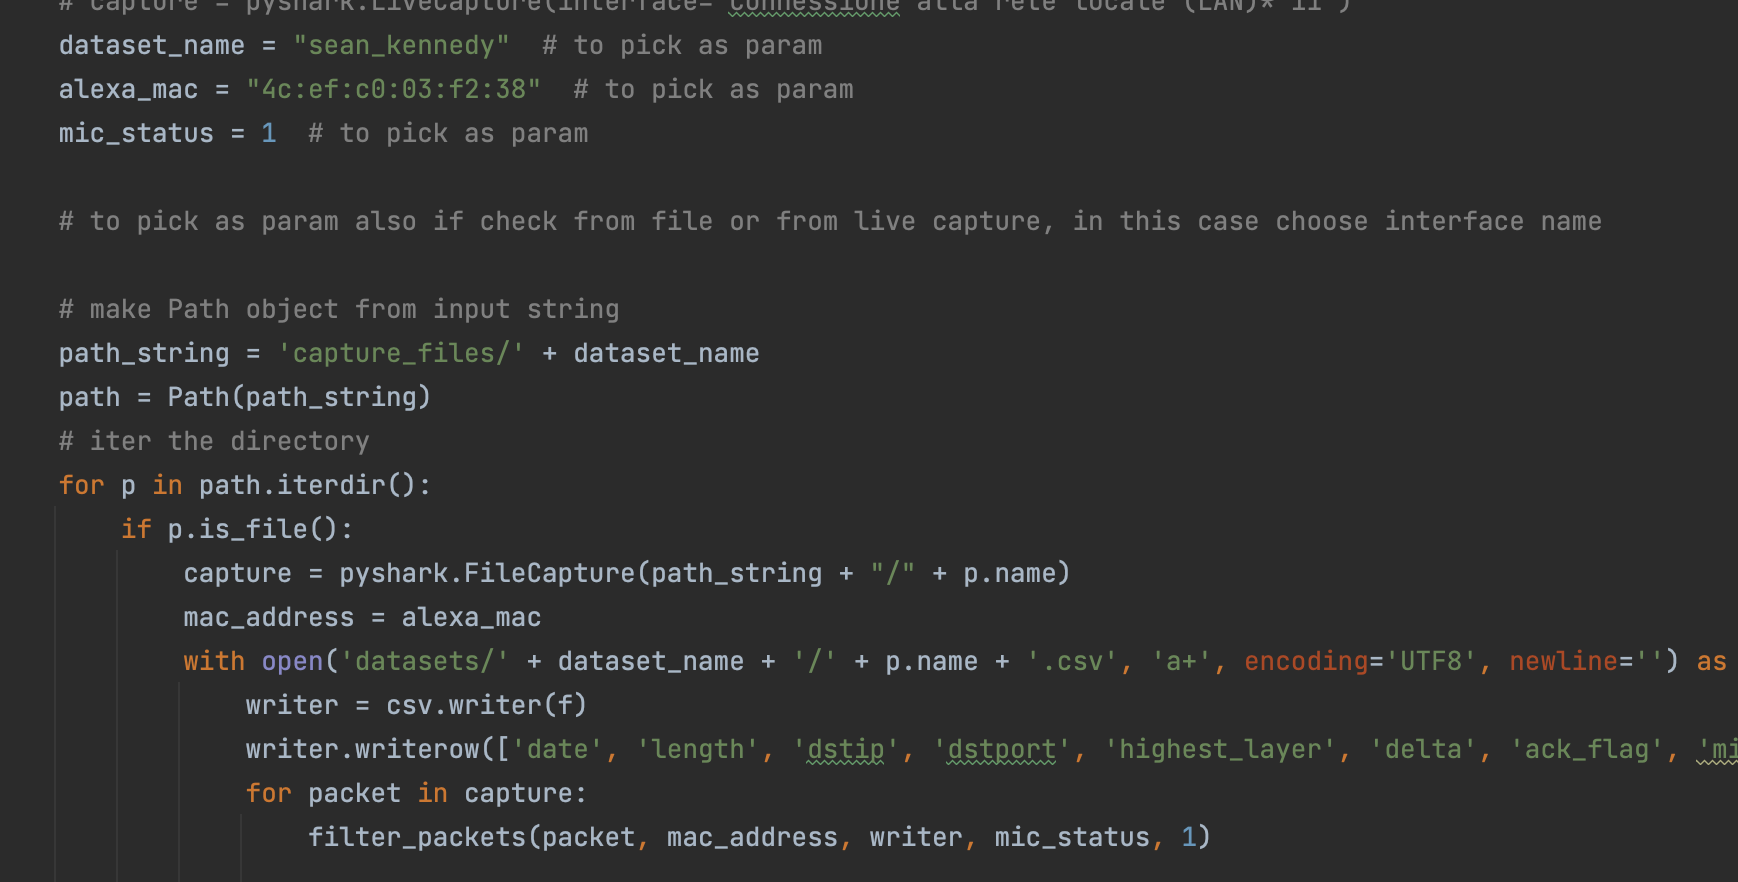
\includegraphics[width=0.8\linewidth]{img/parser.png}
        \caption{Parser able to do live or files capture}
        \label{fig:parser}
    \end{figure}
In this phase no check mechanisms has been take in place; in the following subsection we will see these mechanisms.
\subsection{Data Debt \& Solution}
As introduced in the previous subsection, the data are pushed into a dataset by transforming well-structured data, such as Wireshark packet, into a row of a csv file. In particular, by following the documentation related to the Boi's project, the dataset has the following feature:
\begin{itemize}
\item \textbf{date}: the date in which the packet has been collected, in the format YYYY-MM-DD hh:mm:ss:ms;
        \item \textbf{length}: the length of the packet, it includes just the payload (in case of ack packest it's equal to zero);
        \item \textbf{dstip}: the destination ip, collected to analyze the owner of the server to which the packet is directed;
        \item \textbf{dstport}: the destination port;
        \item \textbf{highest\_layer}: the protocol used, in order to parse the protocol into an integer we will use the following mapping:
        \begin{itemize}
            \item 0 - SSL
            \item 1 - TCP
            \item 2 - DATA
            \item 3 - HTTP
        \end{itemize}
        Notice that all the packets that use other protocol are discarded since they have no meaning for our purpose;
        \item \textbf{delta}: the time occured from the previous packet of the same stream;
        \item \textbf{ack\_flag}: the acknowledge flag; it is equal to 1 if the packet contains an ack;
        \item \textbf{microphone}: the status of the microphone, it is equal to 1 if the microphone is active, 0 otherwise;
        \item \textbf{content\_type}: the type of content sent, it is valorized only if the packet is sent over SSL;
        \item \textbf{synchronized}: status of synchronization of the device, it is equal to 1 if Echo has been previously associated to an account, 0 otherwise.
\end{itemize}
Different problems have been issued here; in order to guarantee a well-structured dataset, that avoid data debt, we have decided to do some checks on dataset created from capture files.
Following problems have been faced up and solved by applying different techniques:
\begin{itemize}
\item When the script tried to analyze packets from the Haipeng and Sean dataset, it was unable to classify application data packets since the highest layer used from the version of Echo Dot was TLS instead of SSL. For this reason, a modification to the parser has been applied in order to correctly classify these packets. Furthermore, other modifications have been introduced to notificate the Data Engineer that the parser wasn't able to assign a class to the packet.
\item During the dataset overview various None values have been retrieved on the class column (which is the target class) and on content type feature; we've decided to delete the rows which contains None values on target class and notificate the Data Engineer in order to check the behavior of the parser, and consequentially modify it in order to optimize the classification; while we have decided to put 0 to content type since the packets that have null content type are related to synchronization and acknowledge packets. We avoided the possibility to use Data Imputation techniques to substitute the value of this target class column, since it is the most important column of the dataset.
Anyway, a final check has been introduced if some new technical modification happens to Echo dot communication system.
\end{itemize}
\subsection{Feature Engineering}
After solved problem on structure, quality and integrity of data captured; we will now discuss about the feature engineering process achieved. As first step we checked if data contains feature that are not relevant for the aim of our project - in particular, the date of packet capture and the destination ip seems to be strictly related to the particular instance of the packet; for this reason we removed these feature.
Furthermore, after conducting an analysis that considers the feature distribution, we've decided to remove the synchronization feature since there is no packet captured without synchronization. This clear behavior of \textit{univariate feature removal} is caused by the Echo Dot architecture, which does not admin any data transferring without Amazon account association. This last consideration, let us think that this feature might be directly removed from the feature captured at parsing time since it is totally not relevant.
\section{Methodology}
In order to implement the tool, we've decided to follow each of these steps:
\begin{enumerate}
\item Consider the current state of art in order to retrieve useful informations. This step is important to produce knowledge to better perform the next steps;
\item Analyze the existing datasets to achieve feature engineering;
\item Apply normalization techniques (data cleaning, data balancing);
\item Implementation and training of a ML model by considering different approaches to find the best fit model for our problem. Looking to the context related projects is most likely that we're going to focus on a Neural Network by using Keras;
\item Analyze, monitor and compare the results of each model by using ML Flow tool;
\item Develop a real time tool based on this model.
\end{enumerate}
Clearly, all these steps will be conducted using a MLOps approach.

    \bibliographystyle{plain}
    \bibliography{biblio_ref}

\end{document}
\endinput
%%
%% End of file `sample-sigconf.tex'.
